\section{Why error estimation controls mixture accuracy}
\label{app:proof}
Fitting weights involves two distinct errors: estimating how the models behave
on new inputs and solving the resulting fitting problem numerically.
The following bound separates these contributions for a fixed library and
expected squared relative error. It uses the population matrix $C$ and its
fitting estimate $\widehat C$ from Section~\ref{sec:analysis}.

\begin{proposition}[Error estimation and mixture risk]
\label{prop:bound}
Suppose $\max_{m,n}|\widehat C_{mn}-C_{mn}|\leq\epsilon$, and $\widehat w$ has empirical
objective within $\delta\geq0$ of the simplex minimum. If $w^*$ minimizes $R$ on the simplex, then
\begin{equation}
 R(\widehat w)-R(w^*)\leq 2\epsilon+\delta.
 \label{eq:bound}
\end{equation}
\end{proposition}
Here $\widehat w$ is the fitted weight vector and $w^*$ is the best population
weight vector. The bound limits their squared risk difference using the largest
matrix estimation error $\epsilon$ and the numerical fitting error $\delta$.

\subsection{Proof of Proposition~\ref{prop:bound}}
Let $A=\widehat C-C$. For every simplex vector,
\begin{equation}
 |w^\top Aw|\leq\sum_{m,n}w_mw_n|A_{mn}|
\leq\epsilon\left(\sum_m w_m\right)^2=\epsilon.
\end{equation}
Here $A_{mn}$ is the estimation error for model pair $(m,n)$. Since the weights
are nonnegative and sum to one, this bounds the risk error for every feasible mixture.
Define $\widehat R(w)=w^\top\widehat Cw$, the fitting mean squared relative
error. Applying empirical near optimality gives
\begin{align}
 R(\widehat w)&\leq\widehat R(\widehat w)+\epsilon\\
 &\leq\widehat R(w^*)+\delta+\epsilon\\
 &\leq R(w^*)+\delta+2\epsilon.
\end{align}
The proof compares both sets of weights under the same estimated risk.
The first and third inequalities each contribute at most $\epsilon$ when
moving between fitting and population error. The middle inequality adds
the numerical optimization error $\delta$. For a feasible numerical solution,
convexity also gives the computable first order gap
\begin{equation}
 \delta_{\rm FW}=\nabla\widehat R(\widehat w)^\top\widehat w
                  -\min_m[\nabla\widehat R(\widehat w)]_m,
\end{equation}
Here $\nabla\widehat R(\widehat w)=2\widehat C\widehat w$ is the objective gradient,
and $[\cdot]_m$ selects its component for model $m$. The Frank Wolfe gap
$\delta_{\rm FW}$ bounds the remaining empirical optimization error. It can
diagnose the numerical solve, while the unknown fitting to population
difference still depends on $\epsilon$. The reported tables therefore provide
no population risk certificate.

\subsection{The number of fields determines the ensemble fitting sample size}
Suppose, conditional on the trained library, fitting examples are independent and identically
distributed and satisfy $|[G_i]_{mn}|\leq B$ almost surely for all $m,n$. Hoeffding's inequality
\citep{hoeffding1963} and a union bound give, with probability at least $1-\alpha$,
\begin{equation}
 \max_{m,n}|\widehat C_{mn}-C_{mn}|
 \leq B\sqrt{\frac{2\log(2M^2/\alpha)}{K}}.
\label{eq:hoeffding}
\end{equation}
Here $B$ bounds each error product, $\alpha\in(0,1)$ is the allowed failure
probability, $M$ counts models, and $K$ counts fitting examples. The equation
controls the largest matrix estimation error simultaneously across model pairs.
Combining this standard result with Proposition~\ref{prop:bound} gives a bound in
terms of the number of fitting examples. The assumptions require care.
Related simulations or climate time dependence can violate independence. Large
errors and near zero target norms can weaken boundedness.
We have not established these assumptions for the present datasets.
For $M=9$, $\alpha=0.05$, and $\delta=0$, the resulting excess risk
bounds are $3.596B$, $2.543B$, and $1.798B$ at $K=5,10,20$.
Since every positive semidefinite $G_i$ has entries bounded by $B$, every
simplex risk lies in $[0,B]$. The trivial excess bound $B$ is therefore tighter
at all three budgets. The concentration result explains a dependence on the
number of fields but is not a useful certificate for these experiments.

Let $P$ be the number of values in one field. Replacing the sample size $K$ with $KP$ would
incorrectly count a field's spatial pixels as independent experiments. This
does not prevent a single field from producing a full rank $M\times M$ Gram
matrix when its model error vectors span $M$ dimensions. Statistical sample
size and matrix rank describe different properties of ensemble fitting.

\subsection{Individual accuracy and complementary errors play different roles}
For positive $d_m=\widehat C_{mm}$, minimize $\sum_m d_m w_m^2$ subject to simplex constraints.
Here $d_m$ is model $m$'s fitting mean squared relative error. Stationarity
yields $2d_m w_m=\lambda$, where $\lambda$ enforces the unit sum constraint.
Normalization yields $w_m\propto d_m^{-1}$, giving more weight to smaller errors.
If any $d_m=0$, a minimum is supported on zero error models. The implementation instead uses
the stated numerical floor. Thus inverse MSE weighting solves the diagonal approximation.
The derivation does not require the actual model errors to be independent.

Equation~\eqref{eq:direction} follows by expanding both quadratic expressions and applying
Cauchy Schwarz to each cross term. For comparison, the usual ambiguity identity is
\begin{equation}
 \sum_m w_m\norm{e_m}_Q^2-\norm{\sum_mw_me_m}_Q^2
 =\sum_m w_m\norm{e_m-\sum_nw_ne_n}_Q^2,
\end{equation}
a standard relation in ensemble analysis \citep{krogh1994}. Here $e_m$ is model
$m$'s relative error field for one case, and $\sum_mw_me_m$ is the mixture error.
The right side measures spread around that mixture error and equals the
reduction from averaging the individual squared errors to averaging predictions.
Both identities describe how combining given error fields can help.
Neither establishes that a particular fitting rule will find useful weights.
The risk bound concerns expected squared relative error. It does not directly
bound the difference in mean relative $L^2$ reported for two methods.

\section{Implementation and reproducibility}
\label{app:protocol}
This section follows the workflow from training the individual models to
fitting and evaluating their combination. We first give each model's data use
and training recipe, then describe the numerical weighting rules and the checks
that keep fitting and evaluation separate. The detailed comparison with
the cited architectures follows in Appendix~\ref{app:adaptations}.

\subsection{How each model uses the available data}
\label{app:experts}

\paragraph{Transfer models.}
FiLM FNO, ConvNeXt, and wavelet transfer use LF pretraining followed by HF finetuning
\citep{li2021fno,perez2018,liu2022convnext,tripura2022wno,lyu2023}.
The nominal setting is 2,500 epochs per stage, AdamW, batch size at most 16,
weight decay $10^{-5}$, gradient clipping at 1, cosine learning rate decay to $10^{-6}$,
and initial learning rates $10^{-3}$ (LF) and $3\times10^{-4}$ (HF).
The FNO recipe uses width 64, four blocks, and up to 12 Fourier modes per direction, subject
to the grid cap. WNO uses a single level wavelet implementation with the archived \texttt{db4}
setting. The ConvNeXt field encoder decoder adapts the visual backbone principle
\citep{liu2022convnext}. The release archive retains the original model definitions and grid dependent choices.
These families have different architectures. They are not matched backbone comparisons.

\paragraph{All pairs.}
One FNO \citep{li2021fno} is conditioned on $x$ and normalized source/target fidelity labels.
Pair enumeration is inspired by Poseidon \citep{herde2024}, with the adaptations in
Appendix~\ref{app:adaptations}.
Its pooled training rows contain target fields. A source field is not an input.
The model therefore predicts from parameters and fidelity labels, rather than
transporting one input field to another. HF finetuning follows joint training.
This changes target repetition and optimization cost as well as conditioning.
Matched update controls are needed to isolate the effect of fidelity pair labels.
For paired data, source/target input identity is verified. In the ERA5 adapter,
exact input joins preserve the correspondence of fields and parameters, and HF finetuning uses HF inputs.
The adapter retains each target field with its own parameters, including repeated target
parameters arising from multiple climate sources.

\paragraph{Distribution FNO.}
The field adaptation trains five LF FNO members and a residual FNO. The residual model
receives parameters and the LF mean, standard deviation, and 10th/50th/90th percentile
summaries. Each member and the residual stage uses the nominal 2,500 epoch recipe.
The original FIRE method uses distribution conditioned in context learning with tabular
foundation models \citep{yu2026fire}. Our trained field implementation is an adaptation.
It is distinct from the separate out of fold corrector construction below.

\paragraph{Retrieved field DeepONet.}
The branch input concatenates parameters and an LF field retrieved from the training
library by nearest neighbor in standardized parameter space. The trunk input is the working grid
coordinate. The output is a residual relative to the interpolated LF field.
At training inputs with an exact LF match, retrieval supplies that matched training field. At unseen queries it supplies a neighboring training field. This inherited retrieval mismatch
is not eliminated by the out of fold construction of the other correctors.
The recipe uses width 256, five affine layers of width 256 in each branch and trunk specification, including
the latent output layer, ReLU,
and 125,000 Adam iterations at learning rate $10^{-3}$ for the nominal 2,500 epoch argument.
It is a DeepONet adaptation \citep{lu2021}, not an exact implementation of the composite
multifidelity architecture of \citet{howard2023}.

\paragraph{Reduced basis.}
POD GP uses reduced basis field emulation \citep{higdon2008}. It fits a basis from
HF base training fields and predicts coefficients with a shared
automatic relevance determination RBF Gaussian process. The selected mode count and fitted
hyperparameters are recorded per dataset. The estimator state was not archived originally. The common export reproduces the training only fit and restores physical scaling.
No fine fitting or evaluation field enters the basis construction.
The additional baselines B1, B2, and B11 evaluate multifidelity models built around POD GP emulators,
while this library member deliberately uses HF data only.

\paragraph{Which coarse data each model uses.}
M1, M3, M4, M5, and M6 use the lowest registered LF level. M2 pools fidelity
pairs across the registered levels, while M8 and M9 predict the finest
registered LF level before correction. M7 uses no LF fields.
Thus common training archives do not imply that each model uses the same
coarse level. In ERA5, the transfer and retrieved field recipes use level one,
whereas the iterative correctors use level eight.

\paragraph{Predicted coarse correctors.}
Each paired dataset uses five LF training folds and four members per fold: plain and
heteroscedastic variants, each with two initializations. Base training rows receive their
held out fold's mean. All query cases use the four members from fixed fold zero.
The Slice attention and ConvNeXt correctors use six refinement steps and predicted mean input,
with adaptations of attention and convolution components \citep{wu2024transolver,liu2022convnext}.
Coarse members have 30,000 requested optimizer steps (rounded to whole epochs by the inherited
trainer). The correctors have 6,000 steps with training only validation. They are custom correctors using the components detailed in
Appendix~\ref{app:adaptations}.

\subsection{Mixture optimization}
\label{app:numerics}
The empirical Gram is symmetrized and scaled by
$\max(\operatorname{tr}(\widehat C)/M,10^{-30})$, which leaves the exact minimizer unchanged.
The trace $\operatorname{tr}(\widehat C)$ sums the diagonal errors, so dividing by
$M$ sets a typical error scale for the optimizer.
SLSQP uses the analytic quadratic gradient, box constraints $0\leq w_m\leq1$, the unit sum
constraint, tolerance $10^{-12}$, and at most 300 iterations. Uniform and lowest diagonal
singleton weights initialize separate solves. Finite candidates with unit sum residual below
$10^{-6}$ are clipped to nonnegative values and renormalized. Feasible starting points remain
available. The lowest empirical objective among candidates is retained. These steps check numerical feasibility and the fitted objective.
They do not establish accuracy on new cases.

\paragraph{Supplementary mixture controls.}
Uniform averaging assigns every model weight $1/M$. Top three uniform first
ranks models by their mean relative $L^2$ error on the fitting examples, then assigns
weight $1/3$ to the best three and zero to the rest. A fitted pair enumerates
all model pairs and fits their nonnegative weights summing to one by minimizing
fitting squared relative error. It retains the best pair or singleton under
that same objective. This control tests whether two active models can approximate
the fitted mixture, while still evaluating all candidates during fitting.
Uniform averaging appears in Table~\ref{tab:main}. Top three and fitted pair
results are retained in the numerical supplement rather than the main
comparison tables.

\paragraph{Cost and refitting.}
For fields with $P$ values, forming the error matrices costs $O(KM^2P)$.
Keeping the matrices after streaming predictions requires $O(KM^2)$ storage.
Here $O$ describes how runtime or storage grows with the numbers of fitting
fields $K$, models $M$, and field values $P$.
These costs exclude training and evaluating the models.
If the coarse input procedure later changes, we can predict the same fitting
cases again and refit the weights using their existing fine answers.
This requires new model predictions but no new fine simulations.

\subsection{Keeping surrogate training, ensemble fitting, and evaluation separate}
The fitting examples are additional fine labels beyond the base training
data. Many datasets have 400 coarse and 400 fine base training rows. Each rule
uses the same stated fitting allowance to select an individual model or fit
mixture weights.
Within a partition, fitting and evaluation input hashes are disjoint and the fitting
budgets are nested: the five examples are included in the ten, which are
included in the twenty. This guarantee is within each dataset. Query grouping
across related variants does not remove their shared base training simulations.
Saved weight hashes and per case
errors are retained for replay. Checks independently reproduce original model errors,
the field/Gram quadratic identity, convex feasibility, and the reported aggregate denominators.
Some cases change roles across the three PDE partitions. Their 1,842
evaluation appearances represent 1,505 distinct dataset and row pairs from
query pools containing 3,058 rows across the 21 PDE datasets. These
are not necessarily independent physical cases across related variants.
The partitions therefore do not constitute three untouched experiments.

For Allen Cahn, Cahn Hilliard II, Fisher KPP, and Phase field crystal, each
fidelity supplies 400 training inputs. Their query pools contain 78, 100, 100,
and 100 inputs, respectively. Each partition reserves 16 evaluation cases for
Allen Cahn and 20 for each other dataset, with the remaining inputs forming
the fitting pool. All nine models, B1 to B11, and the three main ensemble rules
use the same dataset version and evaluation identities. Weight files are sealed
before evaluation. Input hashes verify that reserved inputs do not occur in
any fidelity training table. These additions expand the primary comparison to
21 PDE datasets. Error geometry, subset comparisons, and direct loss
controls in Appendices~\ref{app:geometry} and~\ref{app:reanalysis} retain the
original 17 dataset diagnostic subset.

The ERA5 experiment separates fitting/evaluation answers into different files from
training inputs. Query targets in training trees are zero placeholders, and wrappers reject
access to the answer directory while fitting models. A collector regression changes final
answers and verifies that fitted weights do not change. This verifies the implemented separation of answers and weight fitting.
It does not reconstruct all historical researcher access.
Per stage optimizer and random number generator checkpoints allow training to
resume with the same prescribed budget.

Common array grids, target scaling, and row order are checked before mixing. Seven model export
targets agree within relative tolerance $5\times10^{-7}$. The corrector to canonical target
comparison had maximum discrepancy $3.26\times10^{-8}$ in the feature corpus.
Working grid capping uses the registered data adapter, with a maximum side length of 256.
Historical exports use float32, with TF32 disabled for the seven direct models. Error matrix calculations use float64. The two original corrector exports did not record
their TF32 settings. Fresh heat correctors retain their original convolution precision to
pass replay checks. All comparisons use identical cached predictions within their experiment.
These TF32 differences across historical and fresh exports preclude claiming bit identical inference
across hardware or campaigns. ERA5's unweighted grid metric is not an area weighted global metric.
The source arrays do not verify absolute units or time coordinates. Relative
temperature error changes under an additive unit offset, so its value here
should be interpreted as an archive metric rather than a unit independent
measure of climate skill.

\subsection{Model sources, adaptations, and rationale}
\label{app:adaptations}
Each library member combines a field representation with a training and inference
procedure. We describe M1 to M9 individually below, identifying the published
components retained, the changes made for parameter to field prediction, and
the reason for including each model. Several members combine ideas from more
than one paper. The resulting library is an integration of adapted models,
not nine independent reproductions or nine newly proposed architectures.
All accept parameters alone at deployment. Appendix~\ref{app:experts} gives
their training budgets and data use. The rationales below motivate the library's
composition, while the experiments assess its predictions. They do not isolate
the effect of every architectural change.

\paragraph{M1: FiLM FNO transfer.}
The starting components are FNO's learned Fourier mixing \citep{li2021fno},
FiLM's featurewise affine conditioning \citep{perez2018}, and the LF pretraining
followed by HF finetuning strategy of \citet{lyu2023}. We retain spectral
convolutions with local residual paths and adapt the input interface to a
simulation parameter vector. The spatial input contains coordinates only.
At each block, a parameter network generates a scale and shift applied after
group normalization, so the parameters influence features throughout the
network. Related parameter conditioning for PDE emulation is studied by
\citet{shokar2025}. Our model differs from our parameter concatenation FNO references, which
supply parameters as constant spatial channels at the input. The same weights
are first trained on LF fields and then finetuned on HF fields. This combination
tests whether repeated parameter conditioning and a coarse initialization
provide an effective way to generate globally coupled fields.

\paragraph{M2: All pairs FNO.}
M2 retains M1's FNO and FiLM components \citep{li2021fno,perez2018} and adapts
the idea of pair enumeration from Poseidon \citep{herde2024}. Poseidon uses
pairs of states for temporal operator learning. Here the pairs index source
and target fidelities. We append their normalized labels to the parameter
vector, pool the corresponding target fields on a common working grid, and
train one conditional FNO before HF finetuning. The source label specifies a
training pair, but no source field enters the network. Poseidon's architecture,
pretrained weights, and temporal operator are not used. For ERA5, exact input
joins retain each target field with its own parameters. The purpose is to let
one model share information across fidelity tasks before specializing to the
fine field. Pair enumeration also repeats targets and changes optimization
cost, so its effect cannot be attributed to fidelity conditioning alone.

\paragraph{M3: ConvNeXt transfer.}
ConvNeXt supplies the depthwise spatial convolution, channel expansion, and
residual block structure \citep{liu2022convnext}. We place these blocks in an
U shaped encoder and decoder with skip connections \citep{ronneberger2015} and
a dense field output, adapting the image classification backbone to field
generation. The model starts from
coordinates and replaces the usual block normalization with group normalization
and FiLM conditioning on the simulation parameters \citep{perez2018}. Three
downsampling stages and a bottleneck process the field at several resolutions,
with corresponding decoder stages restoring the target grid. LF pretraining
and HF finetuning follow the transfer principle of \citet{lyu2023}. The
rationale is to provide local spatial processing alongside M1's Fourier mixing,
while retaining the same type of parameter conditioning and transfer schedule.

\paragraph{M4: Distribution FNO.}
FIRE conditions a fine correction on summaries of a coarse predictive
distribution using tabular foundation models and in context inference
\citep{yu2026fire}. M4 retains the distribution conditioning idea and replaces
those models with FNOs trained on spatial fields \citep{li2021fno}. Five LF
members predict a coarse field at the query parameters. Their pointwise mean,
standard deviation, and 10th, 50th, and 90th percentiles become spatial input
channels for a residual FNO, together with coordinates and broadcast parameters.
The residual is added to the coarse mean to predict the fine field. Both stages
are trained by gradient optimization, so this implementation does not retain
FIRE's inference without model retraining. The ensemble summaries are features
of prediction variability, not a guarantee of accurate uncertainty estimates. The
rationale is to expose coarse disagreement as well as the mean to the
correction model. This recipe has no out of fold construction and is distinct
from the coarse ensembles used by M8 and M9.

\paragraph{M5: Wavelet transfer.}
WNO motivates learning in wavelet coordinates \citep{tripura2022wno}. We
replace M1's Fourier mixing with a custom single level db4 wavelet transform,
while retaining its coordinate input, FiLM conditioning \citep{perez2018},
local residual paths, and LF to HF transfer schedule \citep{lyu2023}. Within
each wavelet subband, learned weights mix channels at coefficient positions
inside a capped leading block. Other positions pass through unchanged before
the inverse transform. These indices describe positions within a subband,
not a Fourier frequency cutoff. The implementation also handles rectangular
grids, odd grid sizes, and one dimensional grids. It is a custom wavelet
representation rather than an exact reproduction of the published WNO.
Its inclusion tests whether spatially localized wavelet features provide useful
predictions alongside the spectral and convolutional transfer models.

\paragraph{M6: Retrieved field DeepONet.}
DeepONet supplies the branch and trunk representation \citep{lu2021}, while
the multifidelity use of a coarse prediction as a reference is motivated by
\citet{lu2022mf}. We use a Cartesian product DeepONet whose branch receives
the parameters concatenated with a stored LF training field and whose trunk
receives target grid coordinates. A nearest neighbour search in standardized
parameter space selects that field. The network learns a residual relative to
its interpolated version, which is then added back to form the fine prediction.
Retrieval is the deployment adaptation: a new query requires parameters only
and no new coarse solve. The rationale is to exploit a nearby physical field
without first learning a separate coarse surrogate. If an exact LF match exists
at a training input, retrieval supplies that match, whereas an unseen query
uses a neighboring input. This difference in reference quality remains a
limitation. The implemented residual model is also distinct from the composite
multifidelity architecture of \citet{howard2023}.

\paragraph{M7: POD GP.}
Basis emulation represents a large field through a small set of coefficients
\citep{higdon2008}. M7 retains this principle, constructing a POD basis by
singular value decomposition of centered HF training fields. A Gaussian process
maps parameters to each retained coefficient, and the predicted coefficients
are projected back through the basis and added to the training mean field.
Our implementation uses an RBF kernel with automatic relevance determination
and shares covariance hyperparameters across coefficient outputs. It does not
implement the full Bayesian hierarchy of the cited model. M7 is deliberately
fine only: no coarse field enters basis construction, fitting, or inference.
It supplies a compact alternative when the field varies mainly in a few
directions or when learning a coarse correction is less effective than learning
the fine coefficients directly.

\paragraph{M8: Slice attention corrector.}
Transolver motivates grouping spatial cells into learned slice tokens
\citep{wu2024transolver}. We retain pooled spatial summaries but change the
attention operation. Original Transolver normalizes each cell's assignments
across slices, applies attention between slice tokens, and maps back using
the assignments. Our pooling weights instead normalize across cells, and
cell queries attend directly to the pooled slice tokens. The model receives
the current field, coordinates with sinusoidal features, and FiLM conditioning
on the parameters \citep{perez2018}. A coarse surrogate ensemble supplies its
initial state, with out of fold predictions for training cases. A head
initialized to zero predicts additive corrections through six damped updates
with shared weights. Training penalizes spatial squared error and Fourier
magnitude discrepancy at each update, plus a nonzero update when started at
the target field. This encourages an equilibrium without guaranteeing
contraction. The adaptation tests whether pooled global interactions can
refine a predicted coarse field using parameters alone at deployment. Its
attention and iterative recipe differ from the published Transolver.

\paragraph{M9: ConvNeXt corrector.}
M9 retains ConvNeXt's spatial and channel mixing blocks \citep{liu2022convnext}
and adapts them to the same correction task as M8. It uses a custom U shaped
encoder and decoder with skip connections \citep{ronneberger2015}, three
downsampling stages and a bottleneck,
and FiLM parameter conditioning \citep{perez2018}. Unlike M3, which generates
a field from coordinates and parameters after transfer training, M9 receives
the current coarse estimate as a spatial input and outputs an additive update.
Its head is initialized to zero, making the initial refinement the identity.
The coarse ensemble construction, six damped updates, shared weights, and
spatial, spectral, and target state penalties follow the M8 recipe. The rationale
is to offer local processing at several resolutions as an alternative to pooled
attention when correcting the same kind of coarse prediction. This is a
ConvNeXt based iterative corrector, not the original classification model.

The additional baseline adaptations below use the same distinction between a
source idea and a complete published method. In particular, B1, B5, and B8 omit
central probabilistic components of co kriging, DMFAL, and IFC. Their scores
describe the implemented references, not faithful reproductions of those
complete methods. Common evaluation cases make the scores comparable while
leaving architecture and resource effects coupled.

\paragraph{B1, B2, and B11: classical multifidelity field references.}
B1 applies an autoregressive discrepancy idea \citep{kennedy2000} to POD GP field
models. It fits one scalar coupling coefficient in field space, constructs a
separate POD GP for residuals, and combines posterior means at deployment.
This is a plug in approximation rather than joint probabilistic co kriging.
B2 introduces nonlinear dependence on LF coefficients \citep{perdikaris2017}.
Its HF coefficient kernel combines input dependent coupling, an LF coefficient
kernel, and a discrepancy kernel. It shares covariance hyperparameters across
HF outputs and propagates marginal LF uncertainty through Monte Carlo samples.
B11 is a cheaper affine alternative inspired by multifidelity surrogate work
\citep{zhang2018}. One slope and one intercept are fitted jointly over HF training cases and
pixels, using observed LF fields when paired and emulated LF fields otherwise.
They are then applied to the LF POD GP prediction.
It does not fit an affine mapping separately for each mode. Paired training rows
can use observed LF fields, whereas deployment uses predicted LF fields.

\paragraph{B3, B4, and B5: neural fusion references.}
B3 uses the composite correlation idea of \citet{meng2020}. A tanh MLP maps
parameters and coordinates to an LF value. This stage is frozen before linear
and nonlinear HF networks are trained on the original inputs and LF prediction,
with weight decay on the nonlinear branch. B4 follows the composite DeepONet
idea \citep{howard2023}, predicting fixed coarse sensors with an LF DeepONet and
feeding parameters plus sensors to linear and nonlinear HF DeepONets. The LF
stage is frozen and the HF branches are trained jointly in a subsequent stage. B5 takes hierarchical
latent transfer as inspiration from DMFAL \citep{li2022dmfal}. It uses two encoders
and linear field decoders, with the second encoder receiving parameters and the
first latent vector. Joint LF and HF squared losses replace the probabilistic
objective. Both the variational last layer and active acquisition are omitted.
The name latent MF network reflects these substantial departures.

\paragraph{B6 and B7: alternative decoder and probabilistic models.}
B6 uses NOMAD's nonlinear decoding principle \citep{seidman2022}. A parameter MLP
produces a latent vector and a coordinate conditioned MLP decodes the field.
The model is implemented independently, with multifidelity learning supplied by
LF pretraining and HF finetuning. B7 directly imports MFRNP's upstream
\texttt{MultiFidelityModel} \citep{niu2024}. Its adapter changes data loading,
normalization, resizing, and training. A scalar mean and standard deviation from
the first fidelity normalize inputs, while outputs are scaled per fidelity.
The longest grid side is capped at 256, rectangular grids are supported, and
bilinear antialiased resizing replaces the upstream transform. Batch size is
limited by the smallest fidelity, with independent shuffling across fidelities.
When HF training has at most ten examples, all rows are retained and the context
fraction range changes from $[0.20,0.25]$ to $[0.40,0.60]$. Hidden width is 128,
latent width is 64, and there are three hidden layers. Adam uses learning rate
and epsilon of $10^{-3}$. HF likelihood receives weight two and LF likelihood
weight one. Latent summaries are saved from the final training batch. These are
protocol adaptations of an upstream model, rather than a reproduction of its
published experiment.

\paragraph{B8, B9, and B10: fidelity and transfer FNO references.}
B8 forms latent spatial channels with an FNO and mixes them with weights predicted
from $[\ell,\ell^2]$, the fidelity label and its square. These two features
condition the spatial basis weights on fidelity. It uses maximum absolute scaling
per fidelity, the nearest registered scaler for an intermediate fidelity, LF
warm up, and joint LF and HF finetuning. IFC motivates fidelity dependent
representation \citep{li2022ifc}, but its neural ODE and Gaussian process are
absent. The descriptive name fidelity basis FNO makes this distinction explicit.
B9 and B10 are two archived entries for parameter concatenation FNO transfer
\citep{lyu2023}. In the inspected release, their model files are byte identical
and their training scripts differ only in repository paths and reported
identifiers. The labels FNO transfer I and II distinguish saved result entries,
not independent baseline families. Their different saved scores remain
unexplained by the inspected source. Both are retained to make the archived
comparison auditable, but neither their number nor their score difference is
evidence for architectural diversity or a reproducible recipe difference.
For ERA5 and the four additional reaction diffusion datasets, the identical
recipe is fitted once and its predictions are explicitly reused for B10,
with no additional training cost.


\section{Dataset definitions and evaluation scope}
\label{app:roster}
Table~\ref{tab:roster} lists the available base training rows and reserved query counts
for the paper's 22 datasets. Here $d$ counts input parameters, $N_H$ counts fine
training rows, and $N_{L,\min}$ is the smallest LF table, not the sum over all fidelities.
Counts are input table sizes after excluding reserved query inputs from
training. They do not imply that every model has identical target exposure
or optimizer updates. ERA5 uses 55 HF training cases and 17 reserved queries,
comprising ten fitting pool cases and seven evaluation cases. Its smallest
retained LF table has 313 rows. The original archive had 65 HF training rows,
including the ten subsequently reserved for ensemble fitting.
The class column groups PDE datasets and distinguishes ERA5 climate emulation
\citep{hersbach2020,niu2024}.
Roman numerals distinguish entries with the same governing equation.
Poisson II, Heat II, and Navier Stokes use the MFRNP released data
\citep{niu2024}. ERA5 uses the reanalysis target \citep{hersbach2020} assembled
with climate model sources by MFRNP \citep{niu2024}. Other entries were simulated
for this collection and do not inherit the identity of an external benchmark.

\begin{table}[h!]
\centering\footnotesize\setlength{\tabcolsep}{3pt}
\caption{Inventory of the 22 datasets in this paper. Query cases are later partitioned into fitting pools and evaluation
sets. They are not all final test cases in every reported mixture experiment. Citations identify
imported data. Uncited rows use our simulation code, with recipe influences
distinguished from data sources below.}
\label{tab:roster}\resizebox{\linewidth}{!}{\begin{tabular}{lrrrrrll}
\toprule
Dataset & $d$ & Levels & $N_{L,\min}$ & $N_H$ & Query & Work grid & Class \\
\midrule
Darcy & 16 & 3 & 400 & 400 & 100 & $128\times128$ & Elliptic \\
Eikonal & 3 & 2 & 400 & 400 & 100 & $64\times64$ & Elliptic \\
Helmholtz & 2 & 3 & 400 & 400 & 100 & $256\times256$ & Elliptic \\
Poisson I & 5 & 3 & 400 & 400 & 100 & $64\times64$ & Elliptic \\
Poisson II \citep{niu2024} & 5 & 5 & 64 & 64 & 512 & $128\times128$ & Elliptic \\
Pressure Poisson & 2 & 4 & 400 & 400 & 100 & $64\times64$ & Elliptic \\
Heat I & 3 & 3 & 400 & 400 & 100 & $64\times64$ & Diffusion \\
Heat II \citep{niu2024} & 3 & 5 & 1024 & 1024 & 512 & $128\times128$ & Diffusion \\
Cavity & 1 & 4 & 400 & 400 & 100 & $256\times256$ & Convection \\
Navier Stokes \citep{niu2024} & 2 & 2 & 256 & 256 & 256 & $64\times64$ & Convection \\
Rayleigh Bénard & 1 & 2 & 400 & 400 & 100 & $64\times64$ & Convection \\
Burgers & 2 & 3 & 400 & 400 & 100 & $256\times256$ & Shocks \\
Euler & 7 & 3 & 400 & 400 & 100 & $128\times128$ & Shocks \\
Porous medium & 2 & 3 & 400 & 400 & 100 & $256\times256$ & Porous flow \\
Allen Cahn & 19 & 3 & 400 & 400 & 78 & $256\times256$ & Reaction diffusion \\
Cahn Hilliard I & 2 & 2 & 400 & 400 & 100 & $64\times64$ & Reaction diffusion \\
Cahn Hilliard II & 19 & 3 & 400 & 400 & 100 & $256\times256$ & Reaction diffusion \\
Fisher KPP & 50 & 3 & 400 & 400 & 100 & $256\times256$ & Reaction diffusion \\
Phase field crystal & 18 & 3 & 400 & 400 & 100 & $128\times128$ & Reaction diffusion \\
Shallow water & 2 & 3 & 400 & 400 & 100 & $128\times128$ & Waves \\
Wave & 3 & 2 & 400 & 400 & 100 & $80\times80$ & Waves \\
ERA5 \citep{hersbach2020,niu2024} & 12 & 9 & 313 & 55 & 17 & $128\times256$ & Climate \\
\bottomrule
\end{tabular}
}
\end{table}

The class balanced summary uses elliptic (six entries), diffusion (two),
convection (three), shocks (two), porous flow (one), reaction diffusion (five), and waves (two).
ERA5 supplies a
separate climate case outside the PDE class aggregate. These groups are descriptive labels, not independent
samples of all possible PDE families. Heat outputs are space time fields. The label
``field'' does not imply that both axes are spatial.

The simulation recipes adapt selected settings from existing work: Pressure Poisson
uses an analytic construction motivated by \citet{partin2022}, Euler uses a
quadrant setup motivated by The Well \citep{ohana2024}, and Shallow water uses a
radial dam break recipe motivated by PDEBench \citep{takamoto2022}. These are independently
simulated data, not copies of the cited benchmark datasets. Equation or solver
references alone do not establish dataset provenance.

Poisson I and II are related parameterizations of the same equation.
Cahn Hilliard I and II are distinct data definitions with 2 and 19 input
parameters, respectively. Cahn Hilliard II, Allen Cahn, and Fisher KPP use
$64\times64$, $128\times128$, and $256\times256$ fidelity grids. Phase field
crystal uses $32\times32$, $64\times64$, and $128\times128$ grids. Their input
dimensions are 19, 19, 50, and 18, respectively. These four entries broaden the
reaction diffusion class without adding another PDE class.
Helmholtz normalizes field amplitudes, so its prediction task concerns the
normalized fields.

\section{Detailed results for the common nine model comparison}
\label{app:allresults}
\begin{table}[h!]
\centering\footnotesize\setlength{\tabcolsep}{3.3pt}
\caption{All 21 PDE datasets at $K=5$, averaged over three partitions. Errors are relative $L^2$ percentages.
Change is the percentage change of the fitted mixture relative to the selected model. Negative favors
the fitted mixture. A dagger marks the three entries excluded only in the separate audit sensitivity. Imported Poisson II, Heat II, and Navier Stokes fields are from \citet{niu2024}.}
\label{tab:perdataset}\begin{tabular}{lrrrrr}
\toprule
Dataset & \shortstack[r]{Selected\\model\\(\%)} & \shortstack[r]{Inverse\\error\\mixture\\(\%)} & \shortstack[r]{Fitted\\mixture\\(\%)} & All pairs (\%) & Change (\%) \\
\midrule
Darcy & 2.52202 & 2.54663 & 2.3329 & 3.44071 & -7.50 \\
Eikonal & 1.80881 & 1.76493 & 1.76395 & 2.1513 & -2.48 \\
Helmholtz & 6.24593 & 6.88859 & 6.5522 & 3.47758 & +4.90 \\
Poisson I & 0.00684342 & 0.00799632 & 0.00788219 & 0.0387161 & +15.18 \\
Poisson II$^{\dagger}$ & 0.012093 & 0.0125006 & 0.0129128 & 0.535569 & +6.78 \\
Pressure Poisson$^{\dagger}$ & 0.0733517 & 0.0768584 & 0.0802409 & 0.0695322 & +9.39 \\
Heat I & 0.00971632 & 0.0059257 & 0.00620325 & 0.0125158 & -36.16 \\
Heat II & 0.00661984 & 0.00436575 & 0.00435085 & 0.00878319 & -34.28 \\
Cavity & 0.164294 & 0.142087 & 0.141696 & 0.289895 & -13.76 \\
Navier Stokes & 1.6069 & 1.51806 & 1.49667 & 1.68521 & -6.86 \\
Rayleigh Bénard & 0.00300899 & 0.00285748 & 0.00268826 & 0.00915009 & -10.66 \\
Burgers & 0.516186 & 0.512571 & 0.501656 & 0.533461 & -2.81 \\
Euler & 6.09279 & 5.64117 & 5.7324 & 6.07621 & -5.92 \\
Porous medium & 0.0324973 & 0.0262148 & 0.0263209 & 0.0324973 & -19.01 \\
Allen Cahn & 39.4173 & 37.8786 & 34.6281 & 52.667 & -12.15 \\
Cahn Hilliard I$^{\dagger}$ & 12.1614 & 11.2646 & 10.6611 & 12.5249 & -12.34 \\
Cahn Hilliard II & 52.2253 & 47.2139 & 49.259 & 48.3102 & -5.68 \\
Fisher KPP & 2.36416 & 2.53086 & 2.29888 & 3.21564 & -2.76 \\
Phase field crystal & 83.5396 & 83.7529 & 83.3026 & 89.5093 & -0.28 \\
Shallow water & 0.366692 & 0.357465 & 0.388548 & 0.366692 & +5.96 \\
Wave & 4.84073 & 4.39351 & 4.27458 & 6.30928 & -11.70 \\
\bottomrule
\end{tabular}

\end{table}

The main comparison selects an individual model using fine answers in the fitting set,
which are available before deployment. To measure the accuracy that selection
might miss, we also identify the best fixed model within each partition using
evaluation answers. This is a stronger hindsight reference than choosing one
model per dataset after averaging partitions (Appendix~\ref{app:headlines}).
Against this reference, the fitted mixture at $K=5$ has class aggregated ratio
0.933 and dataset aggregated ratio 1.006, with 13 improvements and 6 losses
larger than 1\%. The mixture is better under one aggregation and worse under
the other. Its advantage therefore depends on both the information used to
choose the reference and the way datasets are weighted.

\subsection{Individual models on the mixture evaluation cases}
\label{app:individual}
Tables~\ref{tab:directexperts} and~\ref{tab:remainingexperts} show whether an
ensemble gain reflects the choice of its members or the combination itself.
They report every member on the exact evaluation cases used by the mixtures,
averaging three partitions of models trained with a single seed. We verify
source hashes, split identities, and saved weights before reconstructing the
means. Replaying the selected model and all pairs columns reproduces their
individual errors, and replaying the mixtures reproduces the reported summary.
Appendix~\ref{app:matchedbaselines} applies the same case correspondence checks
to 13 additional baselines. These tables make the existing predictions directly
comparable without adding new training runs or independent confirmation.

\begin{table}[h!]
\centering\footnotesize\setlength{\tabcolsep}{3pt}
\caption{\textbf{Individual direct models, part one.} Mean relative $L^2$ errors in
percent, averaged over the same three partitions as the mixtures. ``Tr.'' denotes
transfer. A dagger identifies the three entries excluded only in the sensitivity
analysis. Table~\ref{tab:perdataset} provides mixture errors on these cases. Imported Poisson II, Heat II, and Navier Stokes fields are from \citet{niu2024}.}
\label{tab:directexperts}\begin{tabular}{lrrrrr}
\toprule
Dataset & FNO tr. & All pairs & ConvNeXt tr. & Distribution & Wavelet tr. \\
\midrule
Darcy & 3.0655 & 3.4407 & 2.7812 & 4.9816 & 2.319 \\
Eikonal & 2.4216 & 2.1513 & 1.8088 & 4.7865 & 2.5878 \\
Helmholtz & 3.3027 & 3.4776 & 4.7905 & 10.923 & 5.0423 \\
Poisson I & 0.041329 & 0.038716 & 0.042677 & 0.061067 & 0.095469 \\
Poisson II$^{\dagger}$ & 0.25584 & 0.53557 & 0.2003 & 25.532 & 0.88061 \\
Pressure Poisson$^{\dagger}$ & 0.059858 & 0.069532 & 0.091778 & 0.087121 & 0.049757 \\
Heat I & 0.016374 & 0.012516 & 0.010498 & 0.009146 & 0.026774 \\
Heat II & 0.013892 & 0.0087832 & 0.0085933 & 0.0066198 & 0.017272 \\
Cavity & 98.522 & 0.2899 & 98.522 & 0.68058 & 3.6019 \\
Navier Stokes & 1.5549 & 1.6852 & 1.5725 & 1.5783 & 2.3304 \\
Rayleigh Bénard & 0.01123 & 0.0091501 & 0.0071484 & 0.003009 & 0.013708 \\
Burgers & 0.54698 & 0.53346 & 100 & 0.50722 & 1.2763 \\
Euler & 6.197 & 6.0762 & 6.7223 & 6.2957 & 7.4318 \\
Porous medium & 0.044848 & 0.032497 & 0.059555 & 0.065384 & 0.12567 \\
Allen Cahn & 52.986 & 52.667 & 42.085 & 45.442 & 41.345 \\
Cahn Hilliard I$^{\dagger}$ & 12.924 & 12.525 & 12.237 & 11.739 & 36.256 \\
Cahn Hilliard II & 46.907 & 48.31 & 51.926 & 50.754 & 60.826 \\
Fisher KPP & 3.206 & 3.2156 & 2.3642 & 2.9788 & 3.83 \\
Phase field crystal & 89.572 & 89.509 & 110.86 & 83.336 & 202.05 \\
Shallow water & 0.42832 & 0.36669 & 0.36239 & 0.87645 & 0.44595 \\
Wave & 6.3561 & 6.3093 & 4.7526 & 11.137 & 5.0408 \\
\bottomrule
\end{tabular}

\end{table}

\begin{table}[h!]
\centering\footnotesize\setlength{\tabcolsep}{3pt}
\caption{\textbf{Individual direct models and predicted coarse correctors, part two.}
The protocol and percentage error units match Table~\ref{tab:directexperts}.
The POD GP uses HF training data only. Individual models are not retrained on
the additional examples used to fit the mixtures. Imported Poisson II, Heat II, and Navier Stokes fields are from \citet{niu2024}.}
\label{tab:remainingexperts}\begin{tabular}{lrrrr}
\toprule
Dataset & DeepONet & POD GP & Slice attn. corr. & ConvNeXt corr. \\
\midrule
Darcy & 31.69 & 3.3687 & 3.4119 & 3.4119 \\
Eikonal & 7.3707 & 3.6293 & 3.7449 & 2.9509 \\
Helmholtz & 29.112 & 7.1006 & 10.938 & 10.805 \\
Poisson I & 9.9155 & 0.0068434 & 0.12793 & 0.083801 \\
Poisson II$^{\dagger}$ & 26.551 & 0.012093 & 0.92135 & 0.79848 \\
Pressure Poisson$^{\dagger}$ & 0.28471 & 0.092156 & 0.30877 & 0.14457 \\
Heat I & 2.2794 & 0.32711 & 0.049389 & 0.014854 \\
Heat II & 1.5823 & 0.3117 & 0.026827 & 0.012149 \\
Cavity & 70.111 & 0.40924 & 2.0623 & 0.16429 \\
Navier Stokes & 4.4092 & 2.7928 & 2.624 & 1.9475 \\
Rayleigh Bénard & 0.099881 & 0.29516 & 0.052884 & 0.019473 \\
Burgers & 4.8839 & 2.5048 & 1.688 & 0.54472 \\
Euler & 8.133 & 6.1492 & 6.0048 & 5.8807 \\
Porous medium & 2.748 & 0.90855 & 0.68074 & 0.0497 \\
Allen Cahn & 102.03 & 55.463 & 41.396 & 38.754 \\
Cahn Hilliard I$^{\dagger}$ & 81.635 & 30.322 & 41.085 & 12.487 \\
Cahn Hilliard II & 99.848 & 64.811 & 55.889 & 47.845 \\
Fisher KPP & 6.4914 & 6.8627 & 2.8586 & 2.8361 \\
Phase field crystal & 120.13 & 83.54 & 85.25 & 85.74 \\
Shallow water & 1.381 & 1.0928 & 1.291 & 0.50161 \\
Wave & 64.227 & 24.944 & 8.3456 & 11.292 \\
\bottomrule
\end{tabular}

\end{table}

\subsection{Class level and fitting budget comparisons}
\label{app:budgets}
The per dataset table shows where each method succeeds or fails.
Figure~\ref{fig:results} asks how these differences change across problem
classes and as more fitting examples become available.
Table~\ref{tab:budgets} gives the corresponding class aggregated ratios.
The models, partitions, and label accounting are the same as in the main
comparison. These summaries describe the fixed fitting rules on each
dataset, rather than a learned rule for choosing models on another dataset.

\begin{figure}[t]
\centering
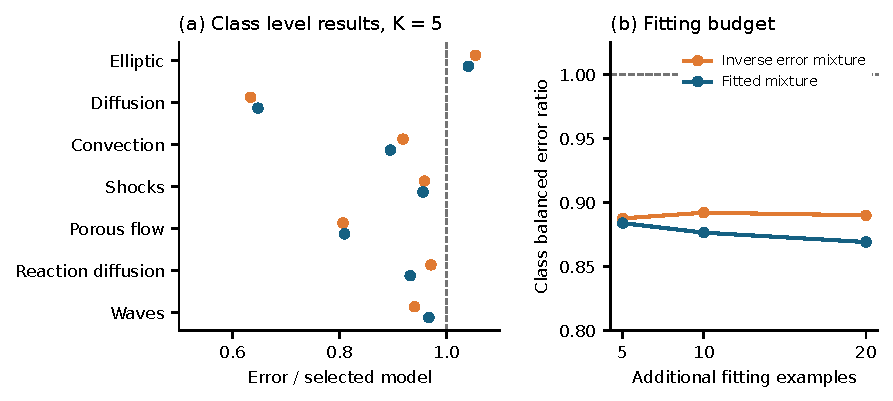
\includegraphics[width=\linewidth]{figures/results_overview.pdf}
\caption{\textbf{Gains vary by problem class and fitting budget.}
Left: geometric error ratios within each class at five fitting examples.
Right: class balanced ratios as the fitting budget increases.
The reference is a single model selected using the same answers.
These points summarize historical partitions, not independent training seeds
with confidence intervals. Appendix~\ref{app:roster} defines the classes.}
\label{fig:results}
\end{figure}

\begin{table}[h!]
\centering\small
\caption{\textbf{Increasing the fitting budget.} Historical class balanced error
ratios. The single model is selected using the same budget as the mixture.}
\label{tab:budgets}\begin{tabular}{rrrr}
\toprule
$K$ & \shortstack[r]{Inverse error mixture /\\Selected model} & \shortstack[r]{Fitted mixture /\\Selected model} & \shortstack[r]{Fitted mixture /\\Inverse error mixture} \\
\midrule
5 & 0.8876 & 0.8840 & 0.9958 \\
10 & 0.8921 & 0.8765 & 0.9826 \\
20 & 0.8900 & 0.8692 & 0.9766 \\
\bottomrule
\end{tabular}

\end{table}

\subsection{Separating library quality from the benefit of averaging}
\label{app:headlines}
For each dataset, the best library reference is the smallest partition averaged
error among M1 to M9. The best additional baseline is the corresponding minimum
among available B1 to B11 results. These are retrospective comparisons using
evaluation answers, not rules for deploying a model. They differ from the
partition specific hindsight control in the original mechanism analysis. All
comparisons below use the same 21 PDE datasets, with complete B1 to B11 coverage.
Table~\ref{tab:paperbaselines} additionally includes ERA5 in its dataset ratios
and Elo ranking.

\begin{table}[h!]
\centering\small
\caption{The two stages of the empirical comparison. Wins and losses require a
relative difference greater than 1\%. Ratios are geometric means. The references
called best use evaluation answers only for this retrospective analysis.}
\begin{tabular}{lrrrr}
\toprule
Comparison & Class ratio & Dataset ratio & Wins & Losses \\
\midrule
Best library / best additional baseline & 0.766 & 0.834 & 15 & 5 \\
Fitted mixture / best library & 0.923 & 0.989 & 13 & 6 \\
Inverse error mixture / best library & 0.927 & 1.002 & 12 & 7 \\
Fitted mixture / best additional baseline & 0.706 & 0.825 & 13 & 7 \\
Fitted mixture / Selected model & 0.884 & 0.923 & 15 & 5 \\
\bottomrule
\end{tabular}

\end{table}

\subsection{Regularized mixture controls}
The supplementary stability experiment tests whether regularizing fixed
weights helps when fitting examples are scarce. It uses the original 17 PDE
dataset subset and the additional Heat I inputs. These are supplementary
controls, separate from the three main rules. Both variants
use the same counted fitting budgets. Shrinkage fits the mixture using
$C_\alpha=\alpha\widehat C+(1-\alpha)\operatorname{diag}(\widehat C)$.
Here $\alpha\in[0,1]$ controls how much of the estimated error interaction is
retained. The operator $\operatorname{diag}$ keeps the diagonal and zeros all
other entries, and $C_\alpha$ replaces $\widehat C$ in the mixture objective.
Thus $\alpha=0$ gives the inverse error mixture and $\alpha=1$ gives the
fitted mixture. Leave one out fitting error selects $\alpha$ from
$\{0,0.25,0.5,0.75,1\}$, and the mixture is refitted on all $K$ fields at the selected value.
This is the LOO shrinkage control. The ridge variant instead minimizes
$w^\top\widehat Cw+\eta s\lVert w-w_{\rm inverse}\rVert_2^2$ on the simplex,
where $s=\max(\min_m\widehat C_{mm},10^{-30})$ and leave one out error selects
$\eta$ from $\{10,1,0.1,0.01,0\}$.
Here $w_{\rm inverse}=w^{\rm inv}$ is the inverse error weight vector, $\eta$ controls the
penalty strength, and $s$ scales it relative to the best individual squared
fitting error. The penalty discourages large departures from inverse weights.
The additional Heat I comparison includes LOO shrinkage under the same fitting
budget, with its errors retained in the numerical supplement.
Such regularization does not supply independent training replicates.

\subsection{Refreshing weights after a coarse input change}
\label{app:refresh}
Fine answers in the fitting set can also be reused when the coarse input procedure
changes. We use the additional Heat I input experiment in
Appendix~\ref{app:additionalheat}, with 128 evaluation cases. We pool the
predicted coarse field to half resolution and reconstruct it before supplying
it to the two correctors. The other seven models remain fixed. Keeping the
inverse weights fitted before this resolution change on the same fitting examples
then gives 0.182726\% error at $K=5$. Repeating predictions for the five fitting examples
with the modified correctors and refitting the weights reduces this to
0.005563\%. The fitted mixture similarly changes from 0.148234\% to 0.005688\%.
Errors average evaluation cases and then fitting selections. The fine
answers are reused, so refreshing the weights requires additional predictions
but no new fine simulations. This controlled perturbation supports
refitting after that change in coarse resolution, without establishing
robustness to arbitrary changes in physics or climate.


\section{Checking comparison coverage}
\label{app:reanalysis}
We test whether the mixture gains depend on comparison coverage using the
original trained models and stored predictions. These diagnostics cover the
original 17 PDE datasets, a subset of the 21 PDE datasets in the primary
comparison. Historical evaluation outcomes had already influenced development
and scope selection, so these analyses are retrospective. The direct relative
$L^2$ fit in Appendix~\ref{app:geometry} is reported as a separate control.

\subsection{Repeating all central comparisons on fixed subsets}
\label{app:subsets}
The 14 dataset subset excludes Poisson II because of inherited numerical
defects, Cahn Hilliard I because its parameters omit realization information,
and Pressure Poisson because its coarse fields are synthetic.
The 15 dataset subset excludes Heat II and Burgers to check sensitivity to
the two B8 entries recovered by checkpoint evaluation. Their
intersection has 12 datasets. Within the revised collection, these subsets use
documented data properties and the recovered entries. None is a newly certified
benchmark. The original seven class assignment is retained, with normalization
over represented classes in each subset.

\begin{table}[h!]
\centering\small\setlength{\tabcolsep}{3pt}
\caption{\textbf{Sensitivity of the principal comparisons.} Each entry gives the
class ratio followed by the equal dataset ratio. Library and baseline denote
the respective best models identified after evaluation. Both mixtures use five fitting examples. Training budgets remain unequal.}
\label{tab:reviewsensitivity}
\resizebox{\linewidth}{!}{\begin{tabular}{lrrrr}
\toprule
Scope & $N$ & Library / baseline & \shortstack[r]{Fitted mixture /\\Selected model} & \shortstack[r]{Inverse error mixture /\\Selected model} \\
\midrule
Diagnostic set & 17 & 0.764 / 0.820 & 0.876 / 0.918 & 0.882 / 0.924 \\
Data quality subset & 14 & 0.747 / 0.810 & 0.873 / 0.900 & 0.875 / 0.908 \\
Without Heat II and Burgers & 15 & 0.790 / 0.865 & 0.872 / 0.935 & 0.872 / 0.940 \\
Intersection & 12 & 0.776 / 0.865 & 0.869 / 0.918 & 0.865 / 0.926 \\
\bottomrule
\end{tabular}
}
\end{table}

The common 15 setting comparison is especially relevant to a claim of beating
individual models. The fitted mixture has ratios 0.916 across classes and 1.020
across datasets to the hindsight best library member. The conclusion changes
with aggregation and coverage even though the fitted mixture improves on
fitting based single model selection.
Table~\ref{tab:reviewsubsets} reports all headline comparisons under each scope.

\begin{table}[p]
\centering\footnotesize
\caption{\textbf{All headline comparisons under each fixed scope.} The four
values of $N$ refer to Table~\ref{tab:reviewsensitivity}. Best library and best
baseline are retrospective minima of partition averaged errors. W, T, and L
use the one percent threshold. Methods use five fitting examples.}
\label{tab:reviewsubsets}\begin{tabular}{rlrrr}
\toprule
$N$ & Comparison & Class ratio & Dataset ratio & W / T / L \\
\midrule
17 & Best library / best additional baseline & 0.764 & 0.820 & 12/0/5 \\
17 & Fitted mixture / best library & 0.915 & 0.992 & 11/1/5 \\
17 & Inverse error mixture / best library & 0.921 & 0.999 & 11/0/6 \\
17 & Fitted mixture / best additional baseline & 0.699 & 0.813 & 10/0/7 \\
17 & Fitted mixture / Selected model & 0.876 & 0.918 & 12/0/5 \\
17 & Inverse error mixture / Selected model & 0.882 & 0.924 & 11/2/4 \\
14 & Best library / best additional baseline & 0.747 & 0.810 & 9/0/5 \\
14 & Fitted mixture / best library & 0.913 & 0.959 & 10/1/3 \\
14 & Inverse error mixture / best library & 0.915 & 0.968 & 10/0/4 \\
14 & Fitted mixture / best additional baseline & 0.682 & 0.777 & 9/0/5 \\
14 & Fitted mixture / Selected model & 0.873 & 0.900 & 11/0/3 \\
14 & Inverse error mixture / Selected model & 0.875 & 0.908 & 10/2/2 \\
15 & Best library / best additional baseline & 0.790 & 0.865 & 10/0/5 \\
15 & Fitted mixture / best library & 0.916 & 1.020 & 9/1/5 \\
15 & Inverse error mixture / best library & 0.916 & 1.026 & 10/0/5 \\
15 & Fitted mixture / best additional baseline & 0.723 & 0.882 & 8/0/7 \\
15 & Fitted mixture / Selected model & 0.872 & 0.935 & 10/0/5 \\
15 & Inverse error mixture / Selected model & 0.872 & 0.940 & 10/1/4 \\
12 & Best library / best additional baseline & 0.776 & 0.865 & 7/0/5 \\
12 & Fitted mixture / best library & 0.914 & 0.987 & 8/1/3 \\
12 & Inverse error mixture / best library & 0.909 & 0.996 & 9/0/3 \\
12 & Fitted mixture / best additional baseline & 0.709 & 0.854 & 7/0/5 \\
12 & Fitted mixture / Selected model & 0.869 & 0.918 & 9/0/3 \\
12 & Inverse error mixture / Selected model & 0.865 & 0.926 & 9/1/2 \\
\bottomrule
\end{tabular}

\end{table}

\begin{table}[p]
\centering\footnotesize
\caption{\textbf{Budget and subset sensitivity of the two mixtures.} Ratios compare with the selected model within each scope.
$N=17,14,15$ denote the historical, audit retained, and common baseline subsets.
All fits share the original models.}
\label{tab:reviewbudgets}\begin{tabular}{rrlrrr}
\toprule
$K$ & $N$ & Rule & Class ratio & Dataset ratio & W / T / L \\
\midrule
5 & 17 & Inverse error mixture & 0.882 & 0.924 & 11/2/4 \\
5 & 17 & Fitted mixture & 0.876 & 0.918 & 12/0/5 \\
5 & 14 & Inverse error mixture & 0.875 & 0.908 & 10/2/2 \\
5 & 14 & Fitted mixture & 0.873 & 0.900 & 11/0/3 \\
5 & 15 & Inverse error mixture & 0.872 & 0.940 & 10/1/4 \\
5 & 15 & Fitted mixture & 0.872 & 0.935 & 10/0/5 \\
10 & 17 & Inverse error mixture & 0.882 & 0.929 & 12/0/5 \\
10 & 17 & Fitted mixture & 0.864 & 0.900 & 12/2/3 \\
10 & 14 & Inverse error mixture & 0.885 & 0.924 & 10/0/4 \\
10 & 14 & Fitted mixture & 0.869 & 0.896 & 10/2/2 \\
10 & 15 & Inverse error mixture & 0.876 & 0.946 & 11/0/4 \\
10 & 15 & Fitted mixture & 0.862 & 0.914 & 10/2/3 \\
20 & 17 & Inverse error mixture & 0.881 & 0.923 & 12/0/5 \\
20 & 17 & Fitted mixture & 0.860 & 0.893 & 13/1/3 \\
20 & 14 & Inverse error mixture & 0.883 & 0.920 & 10/0/4 \\
20 & 14 & Fitted mixture & 0.862 & 0.888 & 11/1/2 \\
20 & 15 & Inverse error mixture & 0.875 & 0.939 & 11/0/4 \\
20 & 15 & Fitted mixture & 0.856 & 0.906 & 12/0/3 \\
\bottomrule
\end{tabular}

\end{table}

\subsection{Duplicate library entries and interpretability of weights}
The prediction source hashes identify the same complete archive for M8 and M9
on Darcy. These two entries therefore do not supply independent
prediction diversity on that dataset. The reanalysis preserves the original
library, including these entries, so it measures the stated historical procedure.
For identical models, many fitted weight allocations have the same combined
field. The inverse error mixture is not invariant to duplicating an entry, since each
copy receives weight before normalization. Effective model count measures
concentration over entries, not the number of distinct mechanisms. A deduplicated
library is a different design whose utility requires a separately specified
evaluation.

\subsection{Additional evaluation inputs for Heat I}
\label{app:additionalheat}
This supplementary experiment evaluates Heat I, one of the 22 datasets, on
additional inputs. It uses 40 new fitting pool cases and 128 new evaluation
cases with the previously trained library. Its scores are reported separately
from the main comparison tables. It evaluates the three main rules and
predates the direct relative $L^2$ fitting control.
\begin{table}[h!]
\centering\small
\caption{\textbf{Additional Heat I inputs.} Mean relative $L^2$ errors in percent. Three
fitting selections share the same 128 evaluation cases and trained models.
Selected model, inverse error mixture, and fitted mixture are the fixed rules in Section~\ref{sec:method}.}
\label{tab:fresh}\begin{tabular}{rrrrr}
\toprule
$K$ & \shortstack[r]{Selected\\model} & \shortstack[r]{Inverse\\error\\mixture} & \shortstack[r]{Fitted\\mixture} & All pairs FNO \\
\midrule
5 & 0.008638 & 0.005300 & 0.005454 & 0.011171 \\
10 & 0.008638 & 0.005286 & 0.005359 & 0.011171 \\
20 & 0.008638 & 0.005270 & 0.005296 & 0.011171 \\
\bottomrule
\end{tabular}

\end{table}


\section{ERA5 evaluation}
\label{app:climateprotocol}
ERA5 contributes the climate dataset \citep{hersbach2020,niu2024}.
Its reported mixture combines nine models trained on inputs disjoint from
fitting and evaluation, with separate fine only FNO and training mean
controls.
ERA5 uses the same nine model library as the PDE experiments, but its climate
results are reported separately from the PDE aggregates. The two correctors
use 49 fine cases for fitting and six for internal validation. Each receives
four coarse predictions per case, with training input identities excluded from
the coarse models producing their features. Observed coarse solutions at the
fine query inputs are not required.

\subsection{ERA5 results}
\label{app:era5}
\begin{table}[t]
\centering\small
\caption{\textbf{ERA5 favors the simple mixture.} Mean relative $L^2$ errors
in percent on seven evaluation cases. Three fitting selections share the same
models trained with a single seed and evaluation inputs. $K=10$ repeats the same ten case pool.}
\label{tab:era5}\begin{tabular}{lrr}
\toprule
Method & $K=5$ & $K=10$ \\
\midrule
Inverse error mixture & 5.8146 & 5.8358 \\
Fitted mixture & 6.4877 & 6.4736 \\
Selected model (POD GP) & 6.7369 & 6.7369 \\
Training mean field & 6.7369 & 6.7369 \\
Uniform mixture & 6.3730 & 6.3730 \\
All pairs FNO & 17.6992 & 17.6992 \\
Fine only FNO & 23.3336 & 23.3336 \\
\bottomrule
\end{tabular}

\end{table}
The target working grid is $128\times256$, compared with the native $721\times1440$
grid. Figure~\ref{fig:overview} displays the ensemble output on the native fine
grid using bilinear interpolation from the working grid. Its fields share one
color scale. The coarse thumbnail is smoothed for illustration, without
changing the training fields or predictions used to compute errors.
The nine evaluated models and separate controls are reported in
Table~\ref{tab:era5experts}. All were retrained on the input disjoint split within ERA5, using a single training seed.
The training mean field is a strong reference: it matches the selected POD GP's error
to displayed precision and outperforms each neural model. The POD GP output is
identical across all 17 fitting/evaluation inputs. Thus its score alone does not
show that it learned a useful response to the climate drivers.

\begin{table}[h!]
\centering\small
\caption{\textbf{All ERA5 models and controls.} Errors are mean relative $L^2$
percentages over the same seven evaluation cases. The separate fine only FNO and
training mean controls are not additional members of the nine model mixture.}
\label{tab:era5experts}\begin{tabular}{lr}
\toprule
Model & Error (\%) \\
\midrule
FiLM FNO transfer & 14.2255 \\
All pairs FNO & 17.6992 \\
ConvNeXt transfer & 20.3962 \\
Distribution FNO & 12.1677 \\
Wavelet transfer & 9.7531 \\
Retrieved field DeepONet & 9.5364 \\
POD GP & 6.7369 \\
Slice attention corrector & 20.3541 \\
ConvNeXt corrector & 8.2403 \\
Fine only FNO control & 23.3336 \\
Training mean field & 6.7369 \\
\bottomrule
\end{tabular}

\end{table}

Three fixed fitting subsets are used. At $K=5$ these select different subsets
of the same ten case pool. At $K=10$ they reuse all ten cases. All fits share the same
seven evaluation inputs and trained models, so the three reported selections are
not independent training replicates. The inverse error mixture has lower
evaluation error than the fitted mixture at both budgets (Table~\ref{tab:era5}).

Figure~\ref{fig:era5cases} shows the case level changes from the training mean field.
The inverse error mixture improves six cases and the fitted mixture improves five.
Neither rule improves every case. We report these observations without
significance claims from seven shared evaluation inputs. Source and prediction
hashes were checked for all ten model and control archives. Saved weight hashes
and per case error files reproduce the reported model and mixture errors. Weights were fixed before evaluation answers were opened by the
scoring stage.

\begin{figure}[t]
\centering
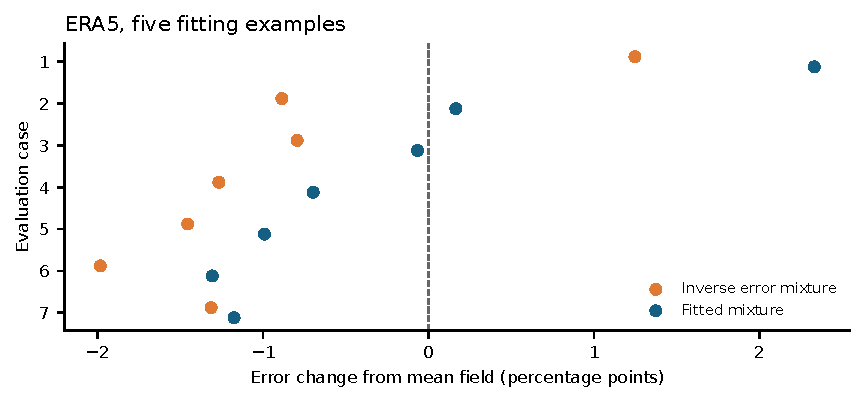
\includegraphics[width=0.88\linewidth]{figures/era5_case_errors.pdf}
\caption{\textbf{ERA5 gains vary across the seven evaluation cases.} Each point is the
change in relative $L^2$ error from the training mean field, in percentage points,
averaged over the three $K=5$ fitting selections. Negative values favor the
mixture. Case numbers identify archive evaluation rows, not calendar dates.}
\label{fig:era5cases}
\end{figure}

\subsection{Label and computation accounting}
The fine data cost is $N_H^{\rm base}+K$, plus any additional HF labels used for
model tuning. Final evaluation fields are excluded from model fitting and
reported separately. Training cost includes every candidate and out of fold
member. Deployment cost includes every active model and shared coarse stage.
A small active ensemble does not remove the cost of candidates already trained
or evaluated during fitting. The available comparisons do not equalize
these costs, and repeated fitting partitions do not estimate variation
across independent training seeds.

\subsection{Scope of the climate prediction task}
The climate inputs describe the supplied simulation drivers. Archive row order
does not establish calendar years or a forecast origin. The evaluation measures
relative error on the registered working grid, without area weighting.
It therefore tests the field emulation pipeline on these inputs and targets.
Broader claims about climate forecasting or policy use would require verified
time coordinates, absolute units, and an application specific evaluation.

\section{Relation to the closest prior systems}
\label{app:prior}
\begin{table}[h!]
\centering\small\setlength{\tabcolsep}{3pt}
\caption{\textbf{How the study relates to existing systems.}
The table compares questions and problem formulations, not measured performance.
These systems were not all run on the same field prediction tasks.}
\begin{tabular}{p{0.22\linewidth}p{0.32\linewidth}p{0.38\linewidth}}
\toprule
Predecessor & Established contribution & Scope of the present investigation \\
\midrule
Engineering surrogate ensembles \citep{acar2009,viana2009} & Optimize validation based mixtures and compare selection with averaging. & Specified neural field library with several fidelity strategies and counted additional fitting examples. \\
Functional output benchmark \citep{brunel2025} & A unified implementation and comparison of multifidelity field emulators. & Heterogeneous neural candidates and ensemble fitting from completed field predictions. \\
Stacking / AutoGluon \citep{wolpert1992,erickson2020} & Library combination and automatic ensemble construction. & Whole field loss and a fixed portfolio of LF use mechanisms. \\
EL MFS / AQBMF \citep{wang2024elmfs,lee2026aqbmf} & Adaptive LF fusion and MF strategy selection. & Heterogeneous field architectures under parameter only deployment. \\
MAESTRO \citep{kim2026maestro} & Multiple LF/discrepancy families with screening and LOOCV selection. & Direct target field models plus correction and fine only alternatives. \\
LANE SI \citep{borisova2024} & Learned combinations of neural and climatological spatial forecasts. & Supplied multifidelity simulations and parametric emulation across problems. \\
HyperNOs \citep{ghiotto2025} & Automated operator training and hyperparameter search. & Fitting based selection among different fidelity use strategies. \\
MFRNP / MF DeepONet \citep{niu2024,howard2023} & Multifidelity field architectures and scientific applications. & A common portfolio selection procedure built from several candidate families. \\
\bottomrule
\end{tabular}
\end{table}
The closest predecessors establish model weighting, automated selection, and
multifidelity field emulation. The present question is how these components
behave together when the candidate models use coarse data in different ways.
The experiments evaluate a common parameter input interface and a counted
fitting budget. Their contribution is evidence about that integrated
workflow, while a direct systems comparison would require matched training,
tuning, and information budgets.

\subsection{Error geometry behind the main analysis}
\label{app:geometry}
Two models with similar individual accuracy can give very different ensemble
gains, depending on where their errors occur and how those errors align.
Classical ensemble analysis makes this dependence explicit
\citep{breiman1996,krogh1994}. For a fixed trained library and population of
inputs, let $C=\E[G(x,y)]$. Because the mixture error is a weighted sum of
individual normalized error fields, its expected squared relative error is
\begin{equation}
 R(w)=\E\left[\frac{\norm{\widehat y_w(x)-y}_Q^2}{\max(\norm y_Q,10^{-8})^2}\right]
 =w^\top Cw.
\label{eq:risk}
\end{equation}
Here $\widehat y_w$ is the combined prediction, $y$ the target, $w$ the model
weights, and $\norm{\cdot}_Q$ the field norm. Expectation $\E$ averages over
input and target pairs, $G(x,y)$ contains their model error products, and $C$
is its mean. The identity computes population squared error from these products.
The diagonal measures individual error and the cross terms measure alignment.
We retain uncentered errors so that shared bias remains part of the risk.
Keeping only a positive diagonal yields the inverse error mixture as the simplex
minimizer before clipping. This is an approximation used to choose weights,
and does not require the actual model errors to be independent.

To separate individual accuracy from complementarity, consider one case and write $r_m=\norm{e_m}_Q$.
If the errors all pointed in the same direction, the squared error of their
weighted sum would be $(\sum_m w_m r_m)^2$.
The difference from the actual mixture is
\begin{equation}
 \left(\sum_m w_m r_m\right)^2-w^\top Gw
 =2\sum_{m<n}w_mw_n\bigl(r_mr_n-\langle e_m,e_n\rangle_Q\bigr)\geq0.
\label{eq:direction}
\end{equation}
Here $r_m$ is the size of error field $e_m$, $G$ is the error product matrix for
the same case, and $m<n$ counts each model pair once. The nonnegative difference
measures how much error alignment matters when the individual error sizes are fixed.
Models can benefit from making errors in different locations or from partially
canceling one another. Negative pairwise correlation is not required.
The inverse error mixture can exploit the same complementarity without fitting cross terms.

\paragraph{The fitting loss can change the preferred weights.}
The effect of the fitting criterion is established in engineering surrogate
ensembles \citep{acar2009}.
The fitted mixture minimizes empirical squared relative error, an estimate of
$R(w)$ in Equation~\eqref{eq:risk}. The reported mean relative $L^2$ error
instead estimates
\begin{equation}
 L(w)=\E\!\left[\sqrt{w^\top G(x,y)w}\right].
\label{eq:reportedrisk}
\end{equation}
Here $L(w)$ is the expected relative $L^2$ error of weights $w$. Taking the
square root for each field before averaging matches the reported metric,
whereas $R(w)$ averages its square.
Jensen's inequality gives $L(w)\leq\sqrt{R(w)}$ for a given $w$ but does not
transfer an excess risk guarantee relative to the minimizer of $L$.
Consider two equally probable scalar cases with normalized errors
$e_A=(0,2)$ and $e_B=(1.1,1.1)$ across cases. Giving A weight $t\in[0,1]$
and B weight $1-t$ yields
\begin{align}
 L(t)&=1.1-0.1t,\\
 R(t)&=1.21-0.22t+1.01t^2.
\end{align}
Here $t$ is model A's weight, and $L(t)$ and $R(t)$ evaluate the unsquared and
squared losses of the same two model mixture. The formulas expose their different optima.
Thus $L$ is minimized at $t=1$, with value one, while $R$ is minimized at
$t=11/101$, where $L=110/101$. Optimizing squared error is approximately
$8.9\%$ worse under the reporting metric in this example. The example also
applies to constant fields and persists with infinitely many fitting cases.

Direct fitting of the reported metric is a convex alternative:
\begin{equation}
 \min_{w\in\Delta_M}\frac{1}{K}\sum_{i=1}^{K}\sqrt{w^\top G_iw}
 =\min_{w\in\Delta_M}\frac{1}{K}\sum_{i=1}^{K}\norm{A_iw}_2,
 \qquad A_i^\top A_i=G_i.
\label{eq:metricfit}
\end{equation}
Here $A_i$ is a matrix factor of the error matrix $G_i$ for fitting example $i$, $\norm{\cdot}_2$
is the Euclidean norm, and $\Delta_M$ enforces nonnegative unit sum weights.
The objective fits the mean relative error over $K$ whole fields directly.
Each summand is a norm of a linear map. Introducing an upper bound $t_i$ for
each field's error, with constraints $\norm{A_iw}_2\leq t_i$, gives a second order cone problem.
This is a standard loss choice, not a new ensemble construction.

\paragraph{What the estimation bound establishes.}
Appendix~\ref{app:proof} shows that entrywise matrix error at most $\epsilon$
and empirical optimization error at most $\delta$ imply excess squared risk
at most $2\epsilon+\delta$ over the best fixed convex mixture for squared
relative error. The deterministic implication requires accurate error
estimation, not independent cases. Independence is needed for the stated
probabilistic sufficient condition, conditional on the frozen library.
That condition concerns whole fields, not individual pixels, and its
assumptions are unverified for this collection. Its numerical bound is weaker
than the trivial bounded risk guarantee at all three reported budgets.
It therefore establishes neither that five fields suffice nor near optimality
under Equation~\eqref{eq:reportedrisk}.

\paragraph{Testing the loss choice while keeping predictions fixed.}
To isolate the fitting objective, we evaluate Equation~\eqref{eq:metricfit} on
all 51 historical partitions at $K=5$, keeping the original nine models,
fitting rows, and evaluation rows. We first reproduce the original selected,
inverse, and fitted error vectors from the stored per case Gram matrices and
verify their input identities. We then fit and save all new weights before
scoring them. The specification was saved before these additional errors were
computed, but the predictions had previously been inspected. This is therefore
a post hoc diagnostic, and the new fit is reported separately from the three main rules.

The epigraph problem uses CVXPY 1.9.2 and Clarabel 0.11.1. All 51 retained solves returned
optimal status with absolute and relative gap tolerances $10^{-10}$ and
feasibility tolerance $10^{-9}$. Scaling by the mean diagonal on the fitting set improves
conditioning without changing the minimizer. Eigenvalues below zero are
clipped only within $10^{-12}$ of spectral scale and every adjustment is
recorded. The most negative relative eigenvalue was approximately
$-1.04\times10^{-18}$. More substantial indefiniteness raises an error.
The largest simplex feasibility residual before nonnegative clipping and
renormalization was $4.15\times10^{-11}$. We also verified the counterexample
above numerically and rejected a deliberately indefinite input matrix.

\begin{table}[t]
\centering\small
\caption{\textbf{Fitting the reported metric directly.} Ratios compare with the
selected model on the original 17 PDE dataset diagnostic subset at five fitting examples.
The fitted mixture uses squared relative error. A win or loss requires
more than a one percent difference after averaging the three partitions for
each dataset. Remaining datasets are within one percent. These are post hoc
results on a fixed library, without independent training replicates.}
\label{tab:losscontrol}
\begin{tabular}{lrrrr}
\toprule
Method & Class ratio & Dataset ratio & Wins & Losses \\
\midrule
Inverse error mixture & 0.882 & 0.924 & 11 & 4 \\
Fitted mixture & 0.876 & 0.918 & 12 & 5 \\
Relative $L^2$ fit & 0.859 & 0.898 & 12 & 5 \\
\bottomrule
\end{tabular}

\end{table}

Direct relative $L^2$ fitting reduces class balanced error by $2.0\%$ and equal
dataset error by $2.1\%$ relative to the original squared error fit
(Table~\ref{tab:losscontrol}). Nine datasets improve by more than one percent,
none worsens by that margin, and eight remain within one percent. Against the
selected model, 12 datasets improve and five worsen. The loss mismatch therefore
has a measurable consequence in these stored predictions. The result motivates
an independent evaluation of this objective choice, without establishing a new
weighting principle or eliminating the limitations of the historical comparison.

